\documentclass[a4paper,12pt]{exam}
	\usepackage{graphicx}
	\usepackage[utf8]{inputenc}
	\usepackage[T1]{fontenc}
	\usepackage{listings}
	\usepackage{color}
	\usepackage{amsmath}
	\usepackage{enumerate}
	\usepackage{caption}
	\usepackage{subcaption}
	\definecolor{dkgreen}{rgb}{0,0.6,0}
	\definecolor{gray}{rgb}{0.5,0.5,0.5}
	\definecolor{mauve}{rgb}{0.58,0,0.82}


\begin{document}
\begingroup 
	  \bf \Large Mecânica Clássica I\\
	  \indent \normalsize André Del Bianco Giuffrida
	\endgroup
	\\ \quad
	\\
	Partindo do problema cuja solução são as seguintes equações:
	\[ x_1 = A \cos{\Big(\frac{\omega_1 - \omega_2}{2} t \Big)}\cos{\Big(\frac{\omega_1 + \omega_2}{2} t \Big)}\]
	
	\[ x_2 = - A \sin{\Big(\frac{\omega_1 - \omega_2}{2} t \Big)}\sin{\Big(\frac{\omega_1 + \omega_2}{2} t \Big)}\]
	E assumindo que esse movimento vem de uma força do tipo $-kx$ podemos chegar a seguinte expressão:
	
	\[ V = - \int F(x)dx = \frac{kx^2}{2}\]
	Utilizando as equações dos movimentos.
	
	\[ V_1 = \frac{kA^2\cos^2{\Big(\frac{\omega_1 - \omega_2}{2} t \Big)}\cos^2{\Big(\frac{\omega_1 + \omega_2}{2} t \Big)}}{2}\]
	
	\[ V_2 = \frac{kA^2 \sin^2{\Big(\frac{\omega_1 - \omega_2}{2} t \Big)}\sin^2{\Big(\frac{\omega_1 + \omega_2}{2} t \Big)}}{2}\]
	
	Plotando fica:
		\begin{figure}[h]
			\centering
			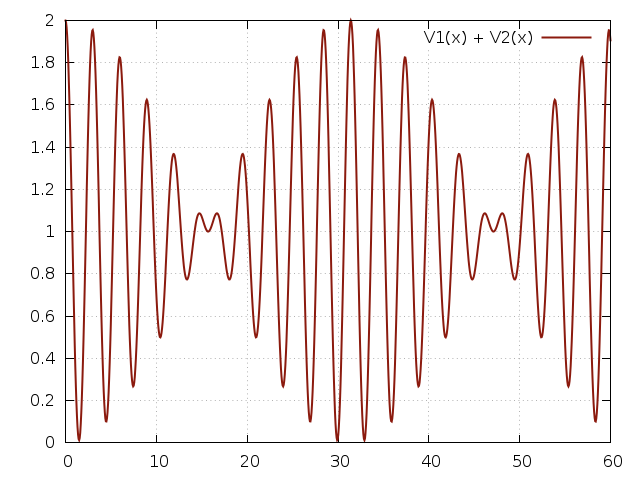
\includegraphics[scale=0.6]{5o0.png}
			\caption{Energia Potencial, $V_1 + V_2$}
		\end{figure}
		
	Agora para a Energia Cinética temos:
	
	\[ T = \frac{m\dot x^2}{2} \]
	
	Usando $\Big(\frac{\omega_1 - \omega_2}{2} \Big) = \omega^{-}$ e $\Big(\frac{\omega_1 + \omega_2}{2} \Big) = \omega^{+}$ para calcular $\dot x$ obtemos:
	
	\[\dot x_1 = - A \Big( \omega^{-} \sin{(\omega^{-} t )}\cos{(\omega^{+} t )} + \omega^{+}\sin{(\omega^{+}t )}\cos{(\omega^{-} t)} \Big)\]
	\[\dot x_2 = - A \Big( \omega^{-} \sin{(\omega^{+} t )}\cos{(\omega^{-} t )} + \omega^{+}\sin{(\omega^{-}t )}\cos{(\omega^{+} t)} \Big)\]
	
	Plotando $T$ obtemos:
		\begin{figure}[h]
			\centering
			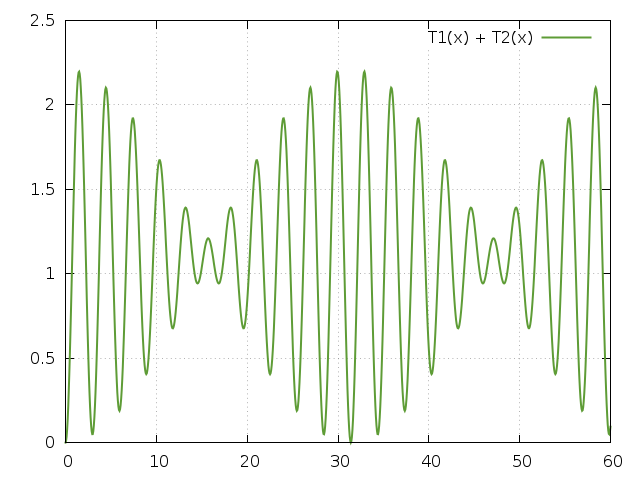
\includegraphics[scale=0.6]{5o1.png}
			\caption{Energia Cinética, $T_1 + T_2$}
		\end{figure}
		
		
		A energia final fica: 
		
		\begin{figure}[h]
			\centering
			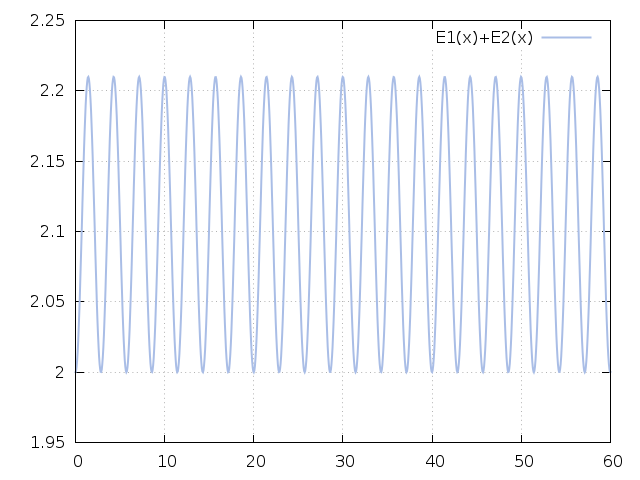
\includegraphics[scale=0.6]{5o2.png}
			\caption{Energia Total, $E1(x) + E2(x)$}
		\end{figure}
		
	\end{document}
